\documentclass[12pt,a4paper]{article}
\usepackage[utf8]{inputenc}
\usepackage{graphicx}
% Document config
\usepackage[letterpaper, margin=1in]{geometry}
\usepackage[spanish]{babel}
\usepackage[utf8]{inputenc}
\usepackage{tikz}
\usepackage{hyperref}
\usepackage{minted,xcolor}
\usemintedstyle{tango}
\usepackage{color}
\usepackage{xcolor}
\usepackage{float}
\usepackage{tcolorbox}
\usepackage[nottoc]{tocbibind}
\usepackage{graphicx}
\usepackage{listings}
\usepackage{lineno}
\usepackage{pdfpages}
\usepackage{titlesec}
\usepackage{fancyvrb}
\usepackage{minted}
\usepackage[utf8]{inputenc}
\usepackage{pdfpages} %para importar paginas de un pdf
\usepackage{multirow}
\addto\captionsspanish{\renewcommand{\listtablename}{Índice de tablas}}		% Cambiar nombre a lista de tablas   
\addto\captionsspanish{\renewcommand{\tablename}{Tabla}}					% Cambiar nombre a tablas
\usepackage{float}		% Para ubicar las tablas y figuras justo después del texto
\usepackage{pdfpages}
\usepackage{enumerate}%listas y viñetas

\usepackage{parskip}
\usepackage{circuitikz}
\usepackage{siunitx}
\usepackage{hyperref}
\hypersetup{
    breaklinks=true, % permitir la ruptura de enlaces a través de líneas
    colorlinks=true, % colorear enlaces
    urlcolor=blue,   % color del enlace URL
}

%%%%%%%%%%%%%%%%%%%%%%%%%%%%%%%%%%%%%%%%%%%%%%%%%%%%%%%%%%%%%%%%%%%%
\title{
{

    \begin{tikzpicture}[overlay, remember picture]
        \node[anchor=north west, %anchor is upper left corner of the graphic
            xshift=3cm, %shifting around
            yshift=-4cm] 
            at (current page.north west) %left upper corner of the page
        {
\includegraphics[height=1.3cm]{logoEIE.png}}; 
    \end{tikzpicture}
    \begin{tikzpicture}[overlay, remember picture]
        \node[anchor=north east, %anchor is upper left corner of the graphic
            xshift=-2.5cm, %shifting around
            yshift=-4cm] 
            at (current page.north east) %left upper corner of the page
        {
\includegraphics[height=1.3cm]{logoUCR.png}}; 
    \end{tikzpicture}
    \Large 
        \textbf{Universidad de Costa Rica}\\
        Facultad de Ingeniería\\
        Escuela de Ingeniería Eléctrica\\~\\ \vspace{2cm}
        \texttt{IE-0624}\\Laboratorio de Microcontroladores \\
    }
    ~\\~\\
    {\LARGE \textbf{Laboratorio \#4: \\ STM32: GPIO, ADC, comunicaciones, Iot \vspace{0cm}}}}
    
\author{Fernando Jiménez Ureña B74020\\ Kristel Herrrera Rodríguez C13769}
\\
\date{II ciclo\\Octubre 2023 } 

%%%%%%%%%%%%%%%%%%%%%%%%%%%%%%%%%%%%%%%%%%%%%%
\usepackage{fancyhdr}
\pagestyle{fancy}
\setlength{\headheight}{14.49998pt}

\lhead{IE0624-Laboratorio de Microcontroladores}
\chead{}
\rhead{Laboratorio \#4}
\lfoot{Universidad de Costa Rica}
\cfoot{\thepage}
\rfoot{Escuela de Ingeniería Eléctrica}
%%%%%%%%%%%%%%%%%%%%%%%


%%%%%%%%%%%%%%%%%%%%%%%%%%%%%%%%%%%%%

\begin{document}
%%%%%%%%%%%%%%%%%%%%%%%%%%%%%%%%%%%%%%%%%%%%%%%%%%%%%%%%%%%
\maketitle
\thispagestyle{empty}%%no formato a la portada
\renewcommand{\thepage}{\roman{page}}
\newpage
%%%%%%%%%%%%%%%%%%%%%%%%%%%%%%%%%%%%%%%%5
\renewcommand{\thepage}{\arabic{page}} 
\setcounter{page}{1}

\newpage


%%%%%%%%%%%%%%%%%%%%%%%%%%%%%%%
\newpage
\section{Resumen}

En el presente reporte y laboratorio, se llevó a cabo el diseño y la implementación de un sismógrafo digital utilizando el microcontrolador STM32F429 y la biblioteca libopencm3, con el fin de registrar y estudiar las oscilaciones en el edificio de la Escuela de Ingeniería Eléctrica. El diseño integra la lectura de los ejes (X, Y, Z) del giroscopio y presenta la funcionalidad de habilitar o deshabilitar las comunicaciones por USART/USB. 

Además el sismógrafo tiene la capacidad de monitorear el nivel de la batería, cuyo rango se extiende de 0 a 9 V. En situaciones donde el nivel de batería se aproxima al límite mínimo de operación del microcontrolador (7V), el sistema activa un LED de alarma y envía una notificación de batería baja al dashboard de ThingsBoard.

Los resultados del monitoreo, incluyendo los valores del giroscopio y el nivel de batería, así como el estado de las comunicaciones, son desplegados en una pantalla LCD. Además, se desarrolló un script en Python capaz de leer y escribir al puerto serial/USB, facilitando la transmisión de estos datos a un dashboard en ThingsBoard. Este último se configuró para visualizar la información relevante, proporcionando una interfaz intuitiva y accesible para el análisis de los datos recopilados.

Este laboratorio  permitió ademas la oportunidad de estudiar sobre el internet de las cosas mediante la paltaforma de ThingsBoard, logrando así aprender sobre las aplicaciones de de monitoreo y análisis de datos en tiempo real.










Dirección del repositorio: \url{https://tinyurl.com/bdfb978w}


\newpage

\section{Nota Teórica}
\subsection{Microcontrolador STM32F429}
\subsubsection{Características Generales}
El microcontrolador STM32F429ZIT6 es una unidad potente y versátil basada en el núcleo ARM 32-bits Cortex-M4 con FPU (unidad de punto flotante). Esta unidad RISC opera a una frecuencia de hasta 180 MHz.

\subsubsection{Memoria y Almacenamiento}
El STM32F429ZIT6 posee una memoria flash de 2 MB y una SRAM de 256 KB. Además, cuenta con un SDRAM adicional de 64-Mbit.


\subsubsection{Comunicación y Conectividad}
\begin{itemize}
    \item USB OTG con conector Micro-AB.
    \item Seis LEDs para diferentes propósitos, incluidos USB Comms y Power On.
    \item Dos push-buttons (Usuario y reset).
    \item Header para LQFP144 I/Os.
    \item Funciones USB: Debug, virtual COM y almacenamiento.
    \item 21 interfaces de comunicaciones que incluyen I2C, USART, SPI, SAI y CAN.
    \item Conectividad avanzada USB 2.0.
    \item Sensor de movimiento I3G4250D y giroscopio STM EMS de 3-ejes.
\end{itemize}

\subsubsection{Alimentación y Energía}
El microcontrolador puede ser alimentado a través de USB o una fuente externa de 3V o 5V. Posee características de bajo consumo para aplicaciones de bajo poder.

\subsubsection{Otras Características}
\begin{itemize}
    \item Controlador LCD-TFT.
    \item 3 ADCs de 12-bit.
    \item 2 convertidores D/A de 12-bit.
    \item 17 timers: 12 de 16-bit y 2 de 32-bit que operan a hasta 180 MHz.
    \item Capacidades de debug: SWD y JTAG.
    \item 168 I/Os con capacidad de interrupción.
    \item Interfaz de cámara.
    \item True RNG (generador de números aleatorios).
    \item CRC (verificación de redundancia cíclica).
    \item Controladores DMA.
\end{itemize}
\subsubsection{Diagrama de bloques}
\begin{figure}[H]
    \centering
    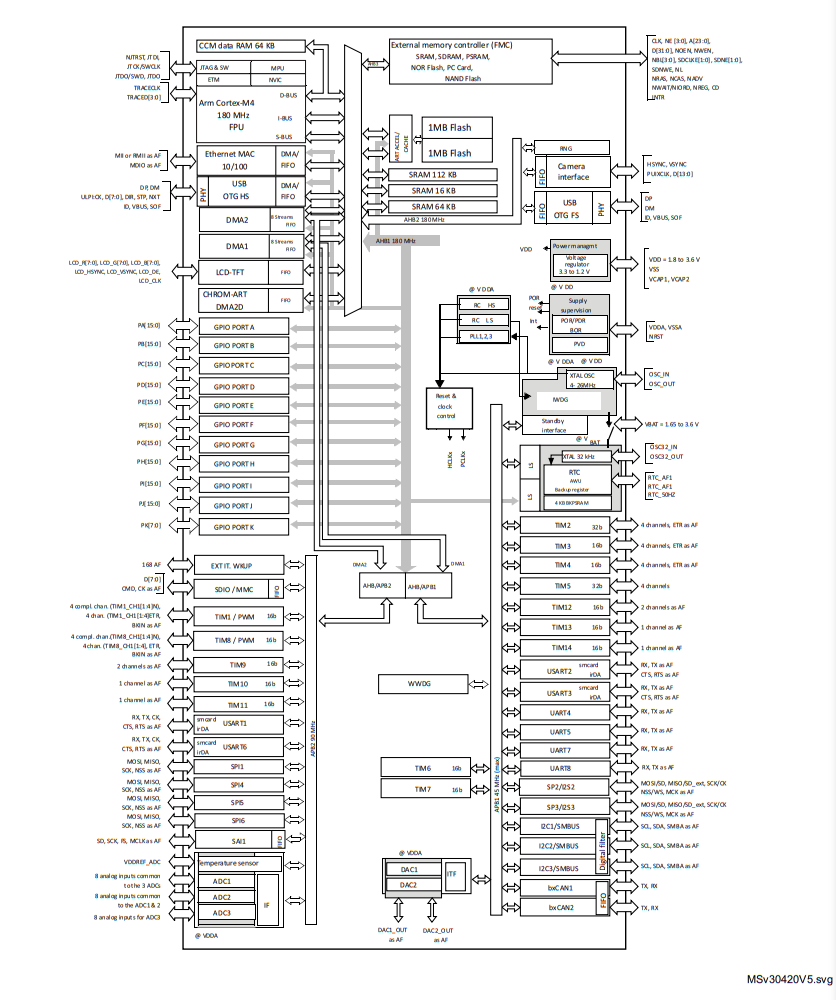
\includegraphics[scale=0.8]{images/Diagrama_bloques.png}
    \caption{Diagrama de bloques. \cite{STM32F429xxDatasheet}}
    \label{fig:bloques}
\end{figure}
\subsubsection{Características eléctricas}
\begin{figure}[H]
    \centering
    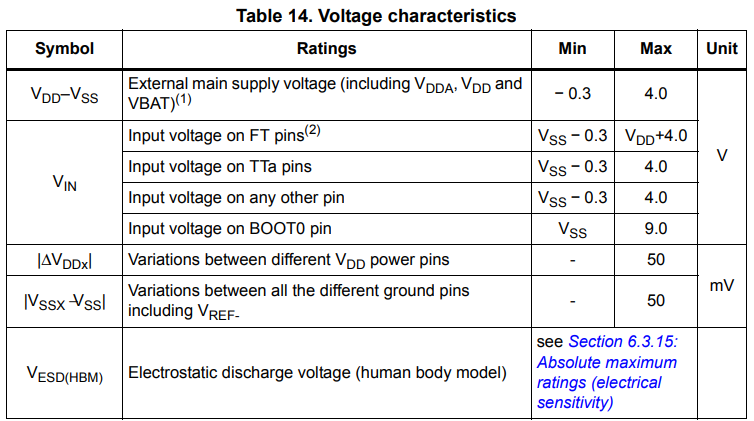
\includegraphics[scale=0.7]{images/Carac_Volt.png}
    \caption{Características de voltaje. \cite{STM32F429xxDatasheet}}
    \label{fig:car_vol}
\end{figure}
\begin{figure}[H]
    \centering
    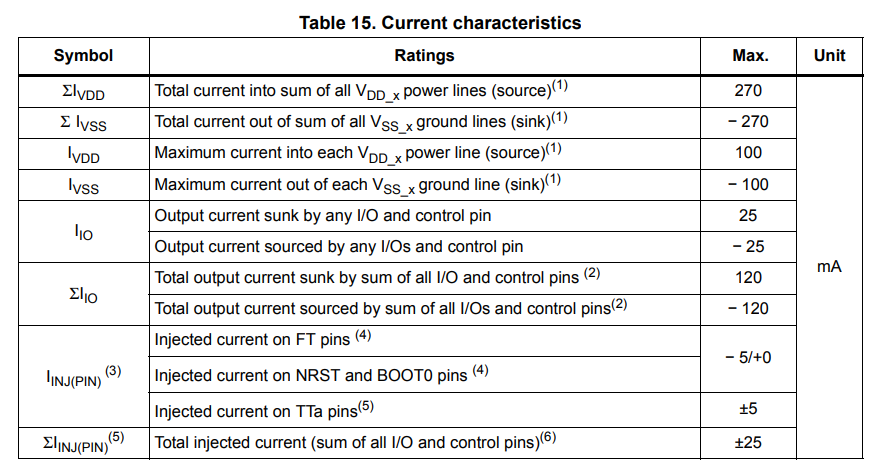
\includegraphics[scale=0.7]{images/Carac_Corr.png}
    \caption{Características de corriente. \cite{STM32F429xxDatasheet}}
    \label{fig:car_cor}
\end{figure}
\subsubsection{Diagrama de pines}
\begin{figure}[H]
    \centering
    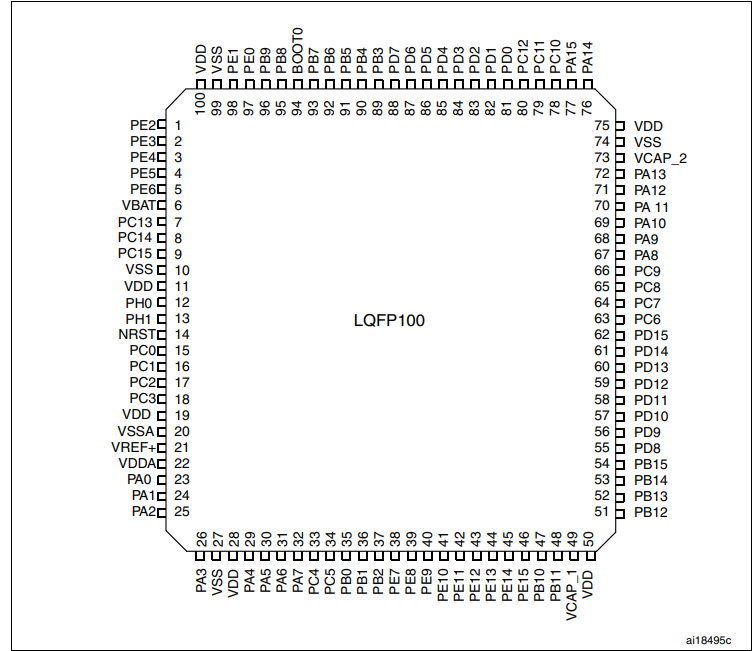
\includegraphics[scale=0.5]{images/diag_pin.png}
    \caption{Diagrama de pines. \cite{STM32F429xxDatasheet}}
    \label{fig:pines}
\end{figure}
\subsubsection{Sensor L3GD20}
El sensor \textbf{MEMS L3GD20} es un giroscopio de tres ejes desarrollado por STMicroelectronics. Este sensor es particularmente destacado por su bajo consumo y capacidad para medir la tasa angular con respecto a un entorno externo. Es decir, puede detectar movimientos de rotación a lo largo de sus tres ejes ortogonales. Para la comunicación con microcontroladores u otros dispositivos, el L3GD20 ofrece interfaces tanto I2C como SPI.

En el contexto del \textbf{STM32F429 Discovery Kit}, este sensor se comunica específicamente a través del protocolo SPI, conectado en la interfaz SPI5 del microcontrolador. La configuración y comunicación con el L3GD20 se realiza mediante instrucciones SPI. Existen varios registros esenciales para su operación:

\begin{itemize}
    \item \texttt{WHOAMI}: Un identificador único que se puede usar para validar la configuración al leer su valor.
    \item \texttt{CTRLREG1}: Se encarga del control de ejes y del modo de energía.
    \item \texttt{CTRLREG2}: Es responsable de la configuración del filtro de paso alto.
    \item \texttt{CTRLREG4}: Define la configuración de los dps y el modo SPI.
\end{itemize}

Para operar el L3GD20 con el STM32F429, es necesario realizar una serie de pasos de configuración, que incluyen habilitar el reloj para el SPI, configurar pines, inicializar y configurar el protocolo SPI y, finalmente, configurar el L3GD20 a través de la interfaz SPI.
\subsubsection{Pantalla y Gráficos}
El microcontrolador tiene un controlador LCD-TFT integrado y está equipado con una pantalla TFT LCD de 2.4" QVGA.

La \textbf{Pantalla LCD/TFT ILI9341} es una pantalla táctil a color con una resolución de 240x320 píxeles. Esta pantalla utiliza el controlador gráfico ILI9341 y un controlador táctil XPT2046 para la detección de toques. A nivel de comunicación, esta pantalla ofrece interfaces I2C y SPI, y en el contexto del \textbf{STM32F429 Discovery Kit}, se comunica específicamente a través de la interfaz SPI5. Como con otros dispositivos periféricos, la configuración y comunicación con el ILI9341 se realiza mediante instrucciones SPI.

El controlador STM32F429 incluye características específicas para el manejo de pantallas, como\cite{STM32F429xxDatasheet}:

\begin{itemize}
    \item Interfaz paralela LCD en modos 8080/6800.
    \item Controlador LCD-TFT con resolución completamente programable, capaz de manejar hasta un ancho de 4096 píxeles, una altura de 2048 líneas y un reloj de píxeles de hasta 83 MHz.
    \item Capacidades para interfaz con la mayoría de los controladores gráficos LCD, soportando los modos Intel 8080 y Motorola 6800.
    \item Controlador de pantalla LCD-TFT que proporciona una salida RGB paralela digital de 24 bits, compatible con una amplia gama de paneles LCD y TFT hasta resolución XGA (1024x768) con características como:
    \begin{itemize}
        \item Dos capas de visualización con FIFO dedicado (64x32-bit).
        \item Tabla de búsqueda de colores (CLUT) de hasta 256 colores (256x24-bit) por capa.
        \item Hasta 8 formatos de color de entrada seleccionables por capa.
        \item Fusión flexible entre dos capas usando un valor alfa (por píxel o constante).
        \item Parámetros programables flexibles para cada capa.
        \item Clave de color (color de transparencia).
        \item Hasta 4 eventos de interrupción programables.
    \end{itemize}
\end{itemize}


\newpage
\subsection{Precios de los componentes}

A continuación se muestran la lista de precios de los componentes utilizados



\begin{table}[h]
\centering
\begin{tabular}{|c|c|}
\hline
\textbf{Componente} & \textbf{Precio (Colones)} \\ \hline
    STM32F429   &  24890.09                   \\ \hline
    Resistencias $680 \Omega$   &  75                   \\ \hline
    Resistencia $3.3 K\Omega$   &  35                   \\ \hline
    Resistencia $5.1 K\Omega$   &  55                   \\ \hline
    Batería $9 V$   &  2395                   \\ \hline
    
    

\end{tabular}
\caption{Precio de los componentes}
\label{tab:my-table}
\end{table}

\newpage

\section{Desarrollo}

\subsection{Diseño}

Con el diseño implementado los dos botones al presionarse van a conectar el pin D2 a +5V, y  la corriente máxima que estos pines pueden proporcionar es de 40 mA. Sin embargo para asegurar el funcionamiento se limitó la corriente a 30 mA.

El valor de la tensión de los LEDs es de 2.0 V. Por lo tanto, utilizando Ley de Kirchhoff para calcular el valor de las resistencias para el caso de un solo LED:

\begin{equation}
    R = \frac{V_{DD} - V_{LED}}{I_{Max}} = \frac{5 - 2.0}{25 mA} =  120\Omega
\end{equation}

Tomando los valores en bodega de la escuela, se eligieron entonces resistencias de para cada uno de los LEDs de $120 \Omega$. Estas resistencias son de gran importancia para proteger los LEDs.

Además, es de suma importancia notar que un circuito RC se agregó para proteger de los efectos rebote a los botones. Se definió una resistencia de $10 K\Omega$ debido a que proporciona una corriente limitada a través del circuito para reducir el consumo de energía y la carga en la fuente de alimentación, seguidamente el capacitor de 10 nF ofrece un buen equilibrio entre filtrado y velocidad de respuesta de los botones. \cite{drmaker2014debouncing}

El tiempo que transcurre desde que se presiona el pulsador momentáneo hasta que el condensador se carga por completo se puede calcular utilizando la siguiente fórmula:

\begin{equation}
    Tiempo (segundos) = {Valor de R} \cdot {Capacidad del condensador}
\end{equation}

Calculando con los valores que se diseñaron para el circuito:

\begin{equation}
    Tiempo (segundos) = 10 K\Omega \cdot 10 nF
\end{equation}

\begin{equation}
    Tiempo (segundos) = 10 K\Omega \cdot 10 nF
\end{equation}

\begin{equation}
    Tiempo (segundos) = 0.1 s
\end{equation}

Este tiempo permite una respuesta lo suficientemente rápida para que el semáforo peatonal se active después de que el usuario presione el botón, y al mismo tiempo elimina de manera efectiva cualquier rebote en el interruptor

A nivel del código implementado, se puede mencionar que se agregaron ciertas características para poder optimizar el rendimiento y código. Entre ellas destacan el uso de macros para definir valores constantes y representar unidades de tiempo clave.

El uso de macros permiten asignar nombres significativos a valores numéricos, lo que hace que el código sea más legible, reutilizable y fácil de mantener. Además, las macros facilitan la modificación de estos valores en un solo lugar, lo que simplifica la adaptación del comportamiento del semáforo sin necesidad de buscar y cambiar cada instancia numérica en el código. Esta característica puede mejorar la escalabilidad del código, ya que cualquier ajuste necesario en los tiempos de cambio de estado o ciclos del temporizador se puede realizar de manera eficiente y precisa simplemente modificando las macros. 

Además otra implementación importante fue el uso de funciones \textit{inline} para funcionalidades como el parpadeo de las luces del semáforo y la gestión de las interrupciones.  ERste tipo de funciones se utilizan para evitar la sobrecarga de llamadas a funciones y, en su lugar, insertar directamente el código de la función en el lugar donde se invoca. Esto ahorra el tiempo y los recursos que normalmente se consumirían en la llamada y retorno de una función, lo que resulta en un código más rápido y eficiente en términos de rendimiento. \cite{microsoftInlineFunctions}

A continuación se muestran los costos de los componentes utilizados:

\begin{table}[h]
\centering
\begin{tabular}{|c|c|}
\hline
\textbf{Componente}     & \textbf{Precio} \\ \hline
ATtiny4313               & 583 colones    \\ \hline
Resistencia de 120 Ohms & 155 colones     \\ \hline
Botón                   & 150 colones     \\ \hline
Resistencia de 10 KOhms & 120 colones     \\ \hline
10 nF capacitor        & 325 colones     \\ \hline
LED Verde              & 310 colones     \\ \hline
LED Rojo              & 310 colones     \\ \hline
\end{tabular}
\caption{Precio de los componentes}
\label{tab:componentes}
\end{table}

\newpage
\subsection{Funcionalidad del diseño}
El circuito en el simulador se muestra de la siguiente manera:
\begin{figure}[H]
    \centering
    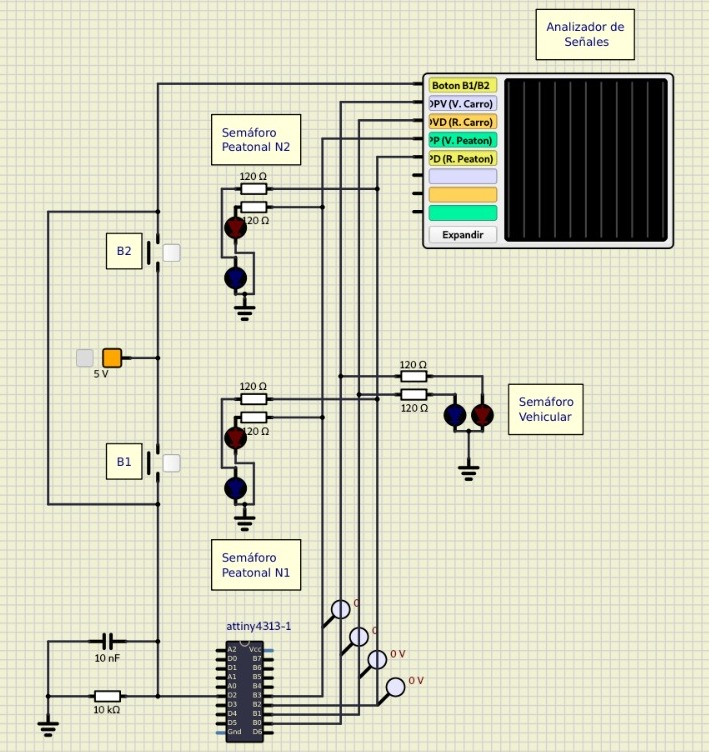
\includegraphics[scale=0.4]{images/Circuito_semaforo.jpeg}
    \caption{Diseño del circuito.}
    \label{fig:semaforo}
\end{figure}

Al poner a funcionar el simulador, se puede observar el estado inicial del semáforo a continuación. Puede notarse que en su estado inicial los semáforos peatonales se encuentran en rojo mientras que el semáforo vehicular en verse

\begin{figure}[H]
    \centering
    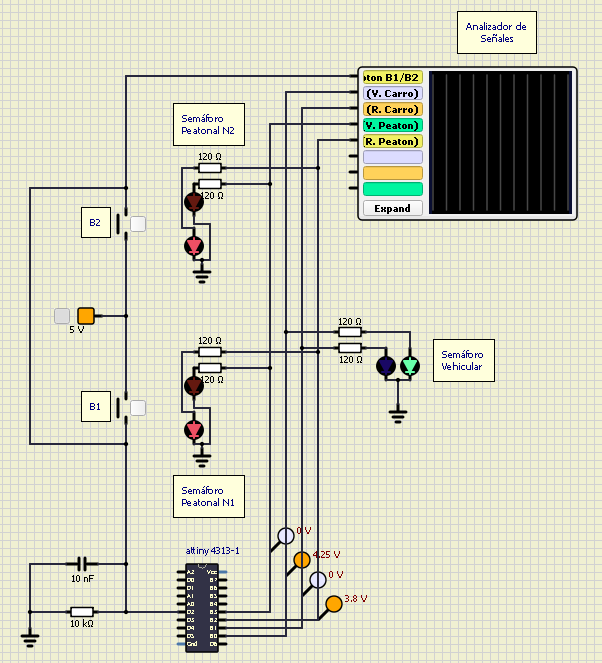
\includegraphics[scale=0.6]{images/uso1.png}
    \caption{Estado inicial del semáforo}
    \label{fig:semaforo2}
\end{figure}

Seguidamente, al presionar cualquiera de los dos botones se puede observar el semáforo peatonal en funcionamiento. El semáforo vehicular pasa a rojo mientras que los peatonales a verde


\begin{figure}[H]
    \centering
    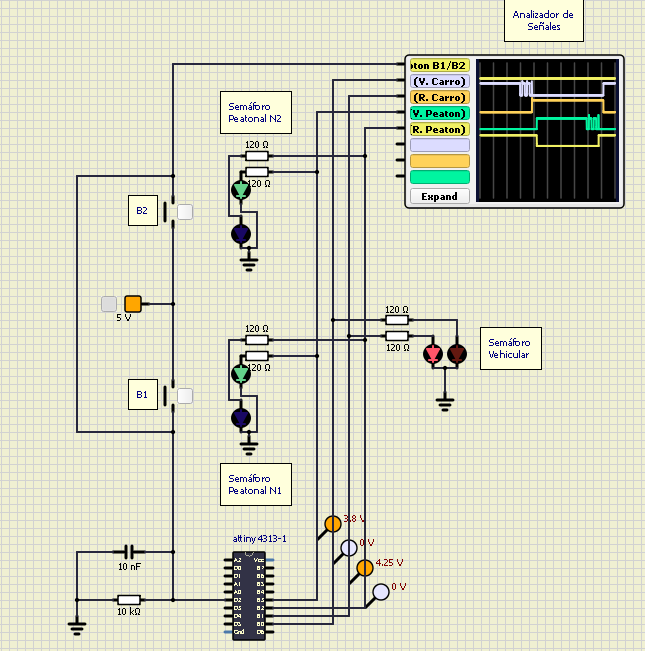
\includegraphics[scale=0.6]{images/uso2.png}
    \caption{Semáforos en funcionamiento}
    \label{fig:semaforo2}
\end{figure}

Finalmente, luego del tiempo definido para el funcionamiento de los semáforos peatonales, éstos vuelven a su estado inicial y el semáforo vehicular vuelve a estar en verde.

\begin{figure}[H]
    \centering
    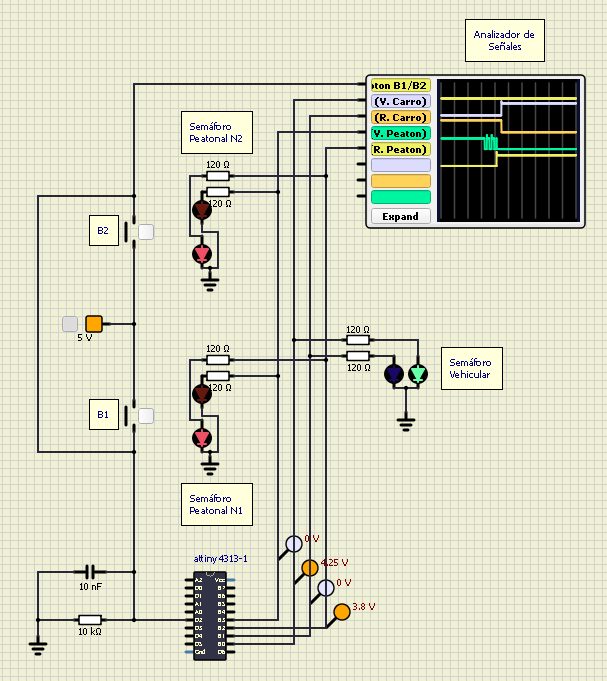
\includegraphics[scale=0.6]{images/uso3.png}
    \caption{Semáforos en funcionamiento}
    \label{fig:semaforo2}
\end{figure}

\newpage

\subsection{Diagrama de estados}
A continuación se presenta el diagrama de estados del proyecto:
\begin{figure}[H]
    \centering
    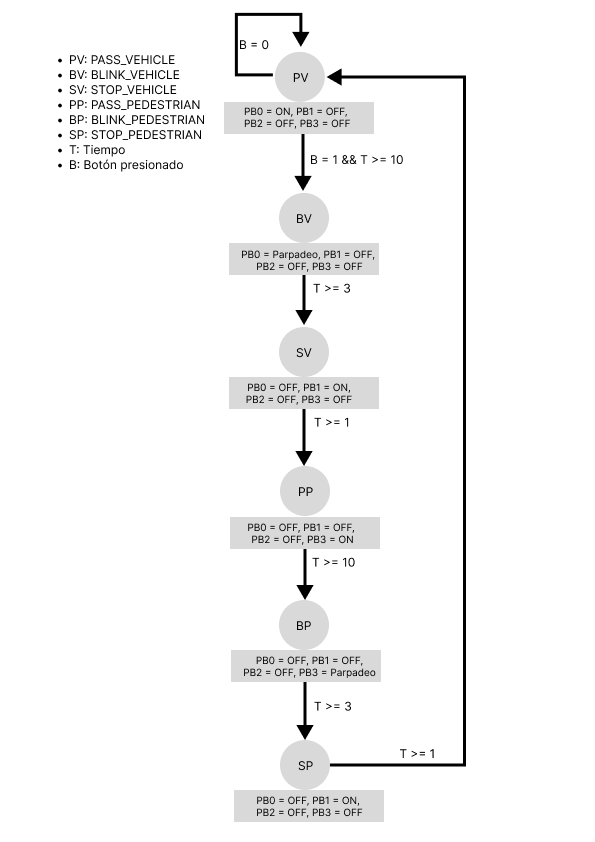
\includegraphics[scale=0.5]{images/Maquina de estados.png}
    \caption{Diagrama de estados.}
    \label{fig:diagrama_estados}
\end{figure}

\newpage
\subsection{Funcionalidad electrónica}
Se colocó un osciloscopio en las salidas de cada pin y en la entrada del botón para mostrar que los cambios en la tensión son los esperados. En la siguiente imagen se puede observar la lectura del osciloscopio.
\begin{figure}[H]
    \centering
    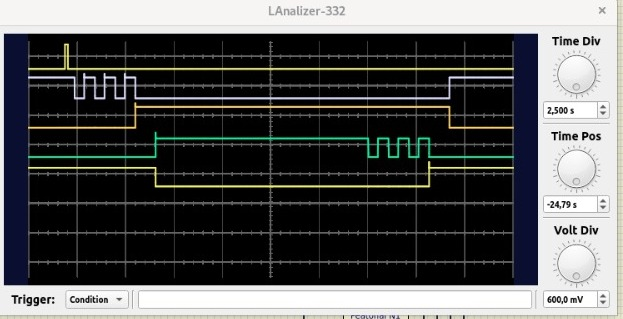
\includegraphics[scale=0.5]{images/Ondas_tiempo.jpeg}
    \caption{Lectura del osciloscopio.}
    \label{fig:diagrama_tiempo}
\end{figure}
Al inicio de las pruebas, todas las salidas se encontraban en un estado lógico bajo (`0'), cumpliendo con las expectativas iniciales. Del mismo modo, el botón de entrada también comenzó en un estado bajo. Cuando se presionó el botón, la señal asociada mostró un flanco ascendente, que activó una transición en la máquina de estados. Durante el experimento, las transiciones entre diferentes estados de las salidas se llevaron a cabo de manera coherente con la definición de la máquina de estados.

Además, se pudo verificar que cada estado se mantenía durante el período de tiempo especificado antes de avanzar al siguiente estado. Es importante destacar que durante las pruebas no se detectaron falsas transiciones ni ruido eléctrico que pudieran afectar la secuencia de estados. Esto indica que el sistema de ``debouncing'' para el botón funciona correctamente, y que la implementación de la máquina de estados funciona de la manera esperada.

\newpage

\section{Conclusiones y Recomendaciones}

\subsection{Conclusiones}

\begin{itemize}

\item El desarrollo y puesta en marcha del sismógrafo se completó con éxito mediante la integración del Microcontrolador STM32F429 Discovery kit y el apoyo de la biblioteca \textit{libopencm3}.

\item La conexión entre el sismógrafo y la plataforma de IoT Thingsboard se estableció exitosamente usando un script de \textit{Python}.

\item La implementación del sistema demostró la versatilidad y potencial de los microcontroladores STM32F429 en aplicaciones de monitoreo y recolección de datos en tiempo real.

\item El uso de la plataforma de IoT Thingsboard permitió una visualización efectiva y en tiempo real de los datos recogidos, mostrando la importancia de las plataformas de IoT en la era digital.

\item La combinación de hardware y software utilizado en este proyecto evidencia que es posible desarrollar sistemas de monitoreo eficientes y asequibles con tecnología disponible en el mercado.


\end{itemize}

\subsection{Recomendaciones}


\begin{itemize}

\item Es recomendable experimentar con diversas combinaciones de resistencias hasta alcanzar la tensión adecuada que garantice el óptimo desempeño del microcontrolador.

\item Para asegurar la correcta lectura de todas las bibliotecas requeridas, se sugiere trabajar con la biblioteca \textit{libopencm3}. Además, es aconsejable implementar y ejecutar el código del sismógrafo dentro de las carpetas de \textit{libopencm3-examples}.

\item Para facilitar la implementación y acelerar el proceso de desarrollo, es beneficioso tomar como referencia los ejemplos previamente establecidos en \textit{libopencm3-examples}.


\end{itemize}

\newpage


\bibliographystyle{IEEEtran}

\bibliography{bibliografia.bib}

\newpage

\section{Apéndices}
\appendix



\end{document}